\documentclass[11pt, oneside]{article}   	% use "amsart" instead of "article" for AMSLaTeX format
\usepackage{geometry}                		% See geometry.pdf to learn the layout options. There are lots.
\geometry{letterpaper}                   		% ... or a4paper or a5paper or ... 
%\geometry{landscape}                		% Activate for for rotated page geometry
\usepackage{parskip}    		% Activate to begin paragraphs with an empty line rather than an indent
\usepackage{graphicx}				% Use pdf, png, jpg, or eps� with pdflatex; use eps in DVI mode
								% TeX will automatically convert eps --> pdf in pdflatex		
\usepackage{amssymb}
\usepackage{amsmath}
\graphicspath{{/Users/telliott_admin/Dropbox/Tex/png/}}

\title{Constrained Optimization: Lagrange multipliers}
%\author{The Author}
\date{}							% Activate to display a given date or no date

\begin{document}
\maketitle
%\section{}
%\subsection{}
\large
This writeup is about the method of Lagrange multipliers.  Suppose we have a function $f(x,y)$ (or $f(x,y,z)$) and we want to maximize it, but the variables are not independent, e.g. $g(x,y) = c$ where $c$ is a constant.  

\subsection*{example 1}

The method of Lagrange multipliers is to find a solution to this equation
\[ \nabla f = \lambda \nabla g \]

If there is a constrained max (or min), it will satisfy this equation.

Suppose

\[ f(x,y) = xy \]
\[ g(x,y) = x + y = 10 \]

This could be the famous maximum area problem where $x$ and $y$ are the sides of a rectangle, the semiperimeter is given, and the objective is to pick $x$ and $y$ to maximize the area.  We see a solution for this in Calculus 1, namely, solve $g$ for one of the variables.

\[ x = 10 - y \]
and substitute:
\[ h(y) = (10-y)y = 10y - y^2 \]
\[ h'(y) = 10 - 2y = 0 \]
\[ h''(y) = - 2 \]
Since the second derivative is $< 0$, this is a maximum, and the solution is $y = 5, x = 5$.

Using the Lagrange method we say
\[ \nabla f = \lambda \nabla g \]
\[ f_x = \lambda g_x \]
\[ f_y = \lambda g_y \]
Plugging in, we obtain two equations

\[ f_x = y = \lambda g_x = \lambda \]
\[ f_y = x = \lambda g_y = \lambda \]
So, clearly $x=y$.

\subsection*{example 2}

Corral gives this problem.  Find the points on the circle $x^2 + y^2 = 80$ that are either closest to or furthest from the point $P = (1,2)$.

The circle equation is out \emph{constraint}.  We need to find an equation for distance, which we will then maximize.
\[ d = \sqrt{(1-x)^2 + (2-y)^2} \]

We can simplify by saying that if $d^2$ is a min or max, then so is $d$.  So now we have

\[ f(x,y) = d^2 = (1-x)^2 + (2-y)^2 = 1 - 2x + x^2 + 4 - 4y + y^2 \]
\[ f_x = -2 + 2x \]
\[ f_y = -4 + 2y \]
\[ g_x = 2x \]
\[ g_y = 2y \]

So 
\[ \nabla f = \lambda \nabla g \]
\[ f_x = \lambda g_x \]
\[ f_y = \lambda g_y \]
Plugging in, we obtain two equations

\[ -2 + 2x = \lambda 2x \]
\[ -4 + 2y = \lambda 2y \]
Solve for $\lambda$ and set them equal

\[ \frac{-4 + 2y}{2y} = \frac{-2 + 2x}{2x} \]
\[ \frac{-2 + y}{y} = \frac{-1 + x}{x} \]
\[ -2x + xy = -y + xy \]
\[ y = 2x \]

Since $x^2 + y^2 = 80$
\[ x^2 + 4x^2 = 80 \]
and so $x= \pm 4$ and the solutions are $(4,8)$, $(-4,-8)$.  Here is the diagram from Corral

\begin{center} 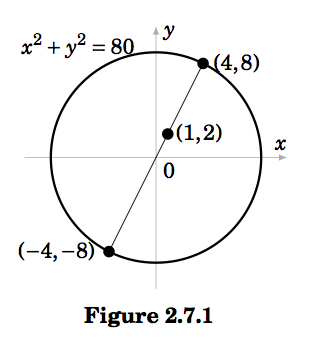
\includegraphics [scale=0.5] {Corral1.png} \end{center}

\subsection*{example 3}
Consider the inverted paraboloid 
\[ z = x^2 + y^2 \]
Now ask, which values $(x,y)$ give a maximum (or minimum) value on the surface, that are also on the line $y = 1 + x$?

Try to visualize what we're asking here.  We have as our surface a kind of elongated and inverted bowl, with its vertex at the origin, opening up.  The vertical plane that cuts through the $x,y$-plane along the given line traces out a curve in its intersection with the surface.  Since the line is symmetric with respect to the origin and the surface is also, I predict that the answer will be that $x = y$.  Let's see.
\[ f(x,y) = x^2 + y^2 \]
\[ \nabla f = \langle \ 2x, 2y \rangle \]
Be sure to re-cast the line equation as a function $g(x,y)$:
\[ g(x,y) = y - x = 1 \]
\[ \nabla g = \langle \ -1, 1 \rangle \]
So we have that
\[ \lambda \ \nabla f = \nabla g \]
This is two equations:
\[ -2x \lambda = 1 \]
\[ 2y \lambda = 1 \]
\[ -\frac{1}{2x} = \frac{1}{2y} \]
\[ -x = y \]
Go back to $g$ to plug in and solve for $x$:
\[ - x - x = 1, \ \ \ x = - \frac{1}{2} \]
and
\[ y = -x = - - \frac{1}{2} = \frac{1}{2} \]
The answer is as we predicted.

\subsection*{example 4}

Auroux gives this problem:  on the curve of the hyperbola $xy=3$, find the point closest to the origin.

The distance to the origin is 
\[ d = \sqrt{x^2 + y^2} \]
but we can simplify things a bit because if $d^2$ is a minimum, then $d$ is a minimum.  So the function we need to minimize is
\[ f(x,y) = x^2 + y^2 \]
subject to the constraint $xy = 3$.

The graph of $f(x,y)$ is a \emph{surface}---a paraboloid with circular cross-section---with apex at $(0,0,0)$, and opening up.  $x^2 + y^2$ is a \emph{level curve} of $f$, at the value $f=a$.

In this figure we have the situation as described, except that  $xy = 1/2$.
\begin{center}
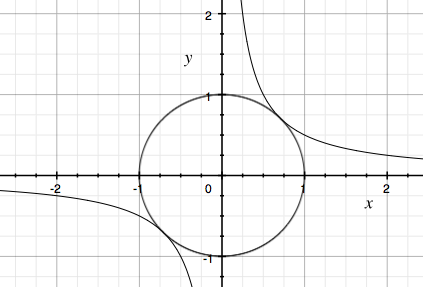
\includegraphics [scale=0.5] {lagrange.png}
\end{center}

The idea of the method is that, at the maximum, the circle just touches the hyperbola.  And at the point of contact, the gradient of the circle function is parallel to the gradient of the hyperbola function, so the two are equal when one is multiplied by a constant that is usually designated $\lambda$.
\[ \nabla f = \lambda \nabla g \]
Before we actually solve this problem, I want to go ahead and look at two more ones (from Paul's Calculus), that are a little easier.  The first is to find the dimensions of a rectangular box with maximum volume, subject to the constraint that the surface area is fixed.

\[ V = xyz \]
\[ A = 2(xy + xz + yz) = constant \]
Now
\[ \nabla V = \ <f_x,f_y,f_z> \]
we have then three equations plus a fourth (the one for area above).
\[ f_x = \lambda g_x = yz = 2 \lambda (y+z) \]
\[ f_y = \lambda g_y = xz = 2 \lambda (x+z) \]
\[ f_z = \lambda g_z = xy = 2 \lambda (x+y) \]
Paul uses a nice trick to solve this.  Take the first two equations, multiply eqn. 1 by x and eqn. 2 by y:
\[ xyz = 2 \lambda x(y+z) \]
\[ xyz = 2 \lambda y(x+z) \]
\[ xy + xz = xy + yz \]
\[ x = y \]
By symmetry, $x=y=z$.

Our second problem is a little easier.  Maximize $f(x,y) = 5x-3y$ subject to the constraint that $x^2 + y^2 = 136$.
\[ f_x = 5 = \lambda g_x = \lambda 2x \]
\[ f_y = -3 = \lambda g_y = \lambda 2y \]
\[ \lambda = 5/2x = -3/2y \]
\[ \lambda = 5/2x = -3/2y \]
\[ 2y/-3 = 2x/5, \ \ \ \ y = -6x/10 \]
To solve this, use the constraint:
\[ x^2 + y^2 = 136 \]
\[ x^2 + (36/100)x^2 = 136 \]
\[ x^2 ( (136/100) ) = 136 \]
\[ x \pm 10, y \pm 6 \]
\[ \lambda = \pm \frac{1}{4} \]
Looking at the original equation, it is obvious that this is a maximum when $x>0$ and $y<0$.
\subsection*{finally solving our problem}

In the original problem, we have
\[ f(x,y) = x^2 + y^2 \]
\[ f_x = 2x \]
\[ f_y = 2y \]
\[ g(x,y) = xy = c \]
\[ \nabla f = \lambda \nabla g \]
so the two equations we get are
\[ 2x - \lambda y = 0 \]
\[ \lambda x - 2y = 0 \]
Auroux uses some linear algebra trickery to solve this.  A matrix equation $A\mathbf{v}=\mathbf{0}$ has solutions other than $\mathbf{v}=0$ only if det(A) = 0.  So that's what we do:
\[ A =
\begin{bmatrix} 
  2  &  -\lambda   \\ 
  \lambda  &  -2  
\end{bmatrix}
\]
The determinant is
\[ -4 + \lambda^2 = 0 \]
\[ \lambda = \pm 2 \]
Using $2x - \lambda y = 0$,for $\lambda = 2$, we obtain $2x-2y=0$ and $x=y$, while for $\lambda = -2$, we obtain $2x+2y=0$ and $x=-y$.  Exactly as you would predict from the figure.  

\end{document}  